\documentclass[12pt,fleqn]{article}\usepackage{../common}
\begin{document}
Bir Coklu Ikisel Dagilim (Multivar. Binary Distribution) ve Hopfield Agi

$$  
P(x;W) = \frac{1}{Z(W)} 
\exp \bigg[ \frac{1}{2} x^T W x \bigg]
$$

Olurluk (likelihood)

$$  
\prod _{n=1}^{N} P(x^{(n)};W) = \frac{1}{Z(W)} 
\exp \bigg[ \frac{1}{2} x^{(n)^T} W x^{(n)} \bigg]
$$

Log olurluk

$$  
\mlabel{1}
\ln \big( \prod _{n=1}^{N} P(x^{(n)};W) \big) = 
\sum _{n=1}^{N} \bigg[ \frac{1}{2} x^{(n)^T} W x^{(n)} - \ln Z(W) \bigg]
$$


Birazdan $w_{ij}$ uzerinden turev alacagiz, $\ln Z(W)$'nin turevi ne
olacak, daha dogrusu $Z(W)$'yi nasil turevi alinir hale getiririz?

$Z(W)$ normalizasyon sabiti olduguna gore, dagilimin geri kalaninin
sonsuzlar uzerinden entegrali (ya da toplami) normalizasyon sabitine
esittir, 

$$ 
Z(W) = \sum_x  \exp \bigg[ \frac{1}{2} x^T W x \bigg]
 $$

$$ 
\ln Z(W) = \ln \bigg[ \sum_x  \exp \big( \frac{1}{2} x^T W x \big) \bigg]
 $$

Log bazli turev alinca log icindeki hersey oldugu gibi bolume gider, ve log
icindekinin turevi alinirak bolume koyulur. Fakat log icine dikkatli
bakarsak bu zaten $Z(W)$'nin tanimidir, boylece denklemi temizleme sansi
dogdu, bolume hemen $Z(W)$ deriz, ve turevi log'un icine uygulariz,


$$ 
\frac{\partial}{\partial w_{ij}} \ln Z(W) = 
\frac{1}{Z(W)}
\bigg[ 
\sum_x \frac{\partial}{\partial w_{ij}} \exp \big( \frac{1}{2} x^T W x \big) 
\bigg]
 $$


$$ 
\mlabel{2}
\frac{\partial}{\partial w_{ij}} \exp \big( \frac{1}{2} x^T W x \big)  = 
\frac{1}{2}  \exp \big( \frac{1}{2} x^T W x \big) 
\frac{\partial}{\partial w_{ij}}x^T W x
$$

(2)'in icindeki bolumu acalim,

$$ \frac{\partial}{\partial w_{ij}}x^T W x = x_i x_j $$

Simdi (2)'ye geri koyalim,

$$ 
=  \frac{1}{2}  \exp \big( \frac{1}{2} x^T W x \big) x_i x_j
 $$


$$ 
\frac{\partial}{\partial w_{ij}} \ln Z(W) = 
\frac{1}{Z(W)}
\bigg[ 
\sum_x \frac{1}{2}  \exp \big( \frac{1}{2} x^T W x \big) x_i x_j
\bigg]
 $$

$$ 
= 
\frac{1}{2}  \sum_x \frac{1}{Z(W)}  \exp \big( \frac{1}{2} x^T W x \big) x_i x_j
 $$

$$ 
= 
\frac{1}{2}  \sum_x P(x;W) x_i x_j
 $$

Artik $\ln Z(W)$'nin turevini biliyoruz. O zaman tum log olurlugun turevi,
(1) uzerinde uygularsak,

$$  
\sum _{n=1}^{N} \bigg[ \frac{\partial}{\partial w_{ij}}  \frac{1}{2} x^{(n)^T} W x^{(n)} - 
\frac{\partial}{\partial w_{ij}}  \ln Z(W) \bigg]
$$


$$  
\sum _{n=1}^{N} 
\bigg[ 
\frac{1}{2} x_i^{(n)^T}x_j^{(n)} - 
\frac{\partial}{\partial w_{ij}}  \ln Z(W) 
\bigg]
$$


\begin{minted}[fontsize=\footnotesize]{python}
import pymc as pm
@pm.potential
def SNLS(X=X):
    logp = -X[0]**2 / X[1]
    logp += -X[1]**2 / X[2]  # or whatever...
    return logp
X = pm.Uniform('X', 0, 1, value=[0.45, 0.24, 0.68])
m = pm.MCMC([X, SNLS])
m.use_step_method(pm.AdaptiveMetropolis, X)
m.sample(100)
\end{minted}

\begin{verbatim}
 [-----------------100%-----------------] 100 of 100 complete in 0.0 sec
\end{verbatim}

\begin{minted}[fontsize=\footnotesize]{python}
pm.Matplot.plot(X)
\end{minted}

\begin{verbatim}
Plotting X_0
Plotting X_1
Plotting X_2
\end{verbatim}


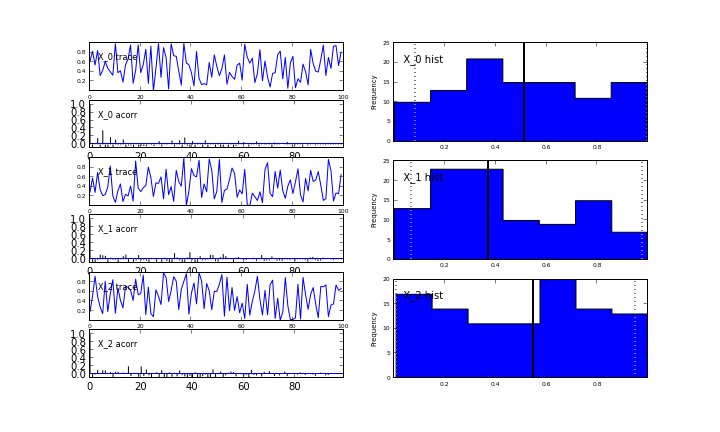
\includegraphics[height=6cm]{X_2.png}




Information Theory, Inference and Learning Algorithms

http://nbviewer.ipython.org/gist/aflaxman/7d946762ee99daf739f1

\end{document}
